% Created by tikzDevice version 0.10.1 on 2016-09-01 16:01:20
% !TEX encoding = UTF-8 Unicode
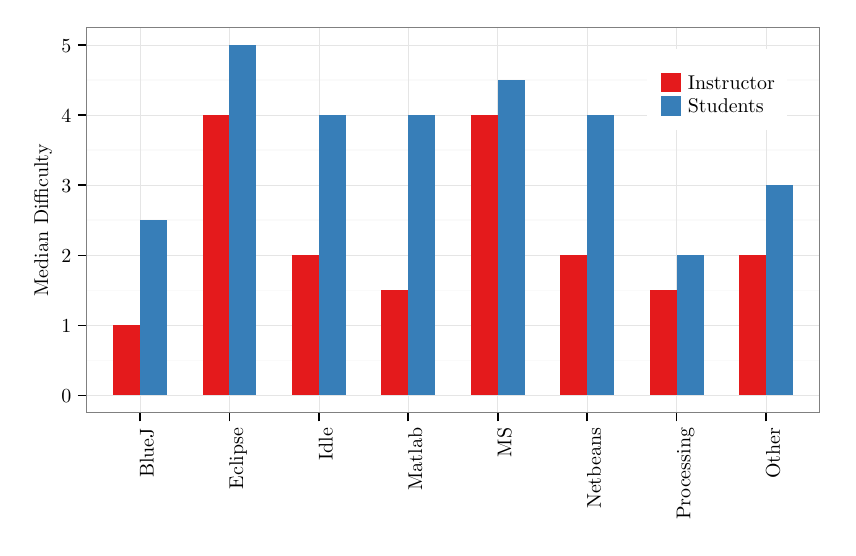
\begin{tikzpicture}[x=1pt,y=1pt]
\definecolor{fillColor}{RGB}{255,255,255}
\path[use as bounding box,fill=fillColor,fill opacity=0.00] (0,0) rectangle (289.08,180.67);
\begin{scope}
\path[clip] (  0.00,  0.00) rectangle (289.08,180.67);
\definecolor{drawColor}{RGB}{255,255,255}
\definecolor{fillColor}{RGB}{255,255,255}

\path[draw=drawColor,line width= 0.6pt,line join=round,line cap=round,fill=fillColor] (  0.00,  0.00) rectangle (289.08,180.68);
\end{scope}
\begin{scope}
\path[clip] ( 21.16, 41.44) rectangle (286.23,180.67);
\definecolor{fillColor}{RGB}{255,255,255}

\path[fill=fillColor] ( 21.16, 41.44) rectangle (286.23,180.67);
\definecolor{drawColor}{gray}{0.98}

\path[draw=drawColor,line width= 0.6pt,line join=round] ( 21.16, 60.42) --
	(286.23, 60.42);

\path[draw=drawColor,line width= 0.6pt,line join=round] ( 21.16, 85.74) --
	(286.23, 85.74);

\path[draw=drawColor,line width= 0.6pt,line join=round] ( 21.16,111.06) --
	(286.23,111.06);

\path[draw=drawColor,line width= 0.6pt,line join=round] ( 21.16,136.37) --
	(286.23,136.37);

\path[draw=drawColor,line width= 0.6pt,line join=round] ( 21.16,161.69) --
	(286.23,161.69);
\definecolor{drawColor}{gray}{0.90}

\path[draw=drawColor,line width= 0.2pt,line join=round] ( 21.16, 47.77) --
	(286.23, 47.77);

\path[draw=drawColor,line width= 0.2pt,line join=round] ( 21.16, 73.08) --
	(286.23, 73.08);

\path[draw=drawColor,line width= 0.2pt,line join=round] ( 21.16, 98.40) --
	(286.23, 98.40);

\path[draw=drawColor,line width= 0.2pt,line join=round] ( 21.16,123.71) --
	(286.23,123.71);

\path[draw=drawColor,line width= 0.2pt,line join=round] ( 21.16,149.03) --
	(286.23,149.03);

\path[draw=drawColor,line width= 0.2pt,line join=round] ( 21.16,174.35) --
	(286.23,174.35);

\path[draw=drawColor,line width= 0.2pt,line join=round] ( 40.55, 41.44) --
	( 40.55,180.67);

\path[draw=drawColor,line width= 0.2pt,line join=round] ( 72.88, 41.44) --
	( 72.88,180.67);

\path[draw=drawColor,line width= 0.2pt,line join=round] (105.21, 41.44) --
	(105.21,180.67);

\path[draw=drawColor,line width= 0.2pt,line join=round] (137.53, 41.44) --
	(137.53,180.67);

\path[draw=drawColor,line width= 0.2pt,line join=round] (169.86, 41.44) --
	(169.86,180.67);

\path[draw=drawColor,line width= 0.2pt,line join=round] (202.19, 41.44) --
	(202.19,180.67);

\path[draw=drawColor,line width= 0.2pt,line join=round] (234.51, 41.44) --
	(234.51,180.67);

\path[draw=drawColor,line width= 0.2pt,line join=round] (266.84, 41.44) --
	(266.84,180.67);
\definecolor{fillColor}{RGB}{55,126,184}

\path[fill=fillColor] ( 40.55, 47.77) rectangle ( 50.25,111.06);
\definecolor{fillColor}{RGB}{228,26,28}

\path[fill=fillColor] ( 30.86, 47.77) rectangle ( 40.55, 73.08);
\definecolor{fillColor}{RGB}{55,126,184}

\path[fill=fillColor] ( 72.88, 47.77) rectangle ( 82.58,174.35);
\definecolor{fillColor}{RGB}{228,26,28}

\path[fill=fillColor] ( 63.18, 47.77) rectangle ( 72.88,149.03);
\definecolor{fillColor}{RGB}{55,126,184}

\path[fill=fillColor] (105.21, 47.77) rectangle (114.90,149.03);
\definecolor{fillColor}{RGB}{228,26,28}

\path[fill=fillColor] ( 95.51, 47.77) rectangle (105.21, 98.40);
\definecolor{fillColor}{RGB}{55,126,184}

\path[fill=fillColor] (137.53, 47.77) rectangle (147.23,149.03);
\definecolor{fillColor}{RGB}{228,26,28}

\path[fill=fillColor] (127.84, 47.77) rectangle (137.53, 85.74);
\definecolor{fillColor}{RGB}{55,126,184}

\path[fill=fillColor] (169.86, 47.77) rectangle (179.56,161.69);
\definecolor{fillColor}{RGB}{228,26,28}

\path[fill=fillColor] (160.16, 47.77) rectangle (169.86,149.03);
\definecolor{fillColor}{RGB}{55,126,184}

\path[fill=fillColor] (202.19, 47.77) rectangle (211.88,149.03);
\definecolor{fillColor}{RGB}{228,26,28}

\path[fill=fillColor] (192.49, 47.77) rectangle (202.19, 98.40);
\definecolor{fillColor}{RGB}{55,126,184}

\path[fill=fillColor] (234.51, 47.77) rectangle (244.21, 98.40);
\definecolor{fillColor}{RGB}{228,26,28}

\path[fill=fillColor] (224.81, 47.77) rectangle (234.51, 85.74);
\definecolor{fillColor}{RGB}{55,126,184}

\path[fill=fillColor] (266.84, 47.77) rectangle (276.54,123.71);
\definecolor{fillColor}{RGB}{228,26,28}

\path[fill=fillColor] (257.14, 47.77) rectangle (266.84, 98.40);
\definecolor{drawColor}{gray}{0.50}

\path[draw=drawColor,line width= 0.6pt,line join=round,line cap=round] ( 21.16, 41.44) rectangle (286.23,180.67);
\end{scope}
\begin{scope}
\path[clip] (  0.00,  0.00) rectangle (289.08,180.67);
\definecolor{drawColor}{RGB}{0,0,0}

\node[text=drawColor,anchor=base east,inner sep=0pt, outer sep=0pt, scale=  0.72] at ( 15.76, 45.29) {0};

\node[text=drawColor,anchor=base east,inner sep=0pt, outer sep=0pt, scale=  0.72] at ( 15.76, 70.60) {1};

\node[text=drawColor,anchor=base east,inner sep=0pt, outer sep=0pt, scale=  0.72] at ( 15.76, 95.92) {2};

\node[text=drawColor,anchor=base east,inner sep=0pt, outer sep=0pt, scale=  0.72] at ( 15.76,121.23) {3};

\node[text=drawColor,anchor=base east,inner sep=0pt, outer sep=0pt, scale=  0.72] at ( 15.76,146.55) {4};

\node[text=drawColor,anchor=base east,inner sep=0pt, outer sep=0pt, scale=  0.72] at ( 15.76,171.87) {5};
\end{scope}
\begin{scope}
\path[clip] (  0.00,  0.00) rectangle (289.08,180.67);
\definecolor{drawColor}{RGB}{0,0,0}

\path[draw=drawColor,line width= 0.6pt,line join=round] ( 18.16, 47.77) --
	( 21.16, 47.77);

\path[draw=drawColor,line width= 0.6pt,line join=round] ( 18.16, 73.08) --
	( 21.16, 73.08);

\path[draw=drawColor,line width= 0.6pt,line join=round] ( 18.16, 98.40) --
	( 21.16, 98.40);

\path[draw=drawColor,line width= 0.6pt,line join=round] ( 18.16,123.71) --
	( 21.16,123.71);

\path[draw=drawColor,line width= 0.6pt,line join=round] ( 18.16,149.03) --
	( 21.16,149.03);

\path[draw=drawColor,line width= 0.6pt,line join=round] ( 18.16,174.35) --
	( 21.16,174.35);
\end{scope}
\begin{scope}
\path[clip] (  0.00,  0.00) rectangle (289.08,180.67);
\definecolor{drawColor}{RGB}{0,0,0}

\path[draw=drawColor,line width= 0.6pt,line join=round] ( 40.55, 38.44) --
	( 40.55, 41.44);

\path[draw=drawColor,line width= 0.6pt,line join=round] ( 72.88, 38.44) --
	( 72.88, 41.44);

\path[draw=drawColor,line width= 0.6pt,line join=round] (105.21, 38.44) --
	(105.21, 41.44);

\path[draw=drawColor,line width= 0.6pt,line join=round] (137.53, 38.44) --
	(137.53, 41.44);

\path[draw=drawColor,line width= 0.6pt,line join=round] (169.86, 38.44) --
	(169.86, 41.44);

\path[draw=drawColor,line width= 0.6pt,line join=round] (202.19, 38.44) --
	(202.19, 41.44);

\path[draw=drawColor,line width= 0.6pt,line join=round] (234.51, 38.44) --
	(234.51, 41.44);

\path[draw=drawColor,line width= 0.6pt,line join=round] (266.84, 38.44) --
	(266.84, 41.44);
\end{scope}
\begin{scope}
\path[clip] (  0.00,  0.00) rectangle (289.08,180.67);
\definecolor{drawColor}{RGB}{0,0,0}

\node[text=drawColor,rotate= 90.00,anchor=base east,inner sep=0pt, outer sep=0pt, scale=  0.72] at ( 45.51, 36.04) {BlueJ};

\node[text=drawColor,rotate= 90.00,anchor=base east,inner sep=0pt, outer sep=0pt, scale=  0.72] at ( 77.84, 36.04) {Eclipse};

\node[text=drawColor,rotate= 90.00,anchor=base east,inner sep=0pt, outer sep=0pt, scale=  0.72] at (110.17, 36.04) {Idle};

\node[text=drawColor,rotate= 90.00,anchor=base east,inner sep=0pt, outer sep=0pt, scale=  0.72] at (142.49, 36.04) {Matlab};

\node[text=drawColor,rotate= 90.00,anchor=base east,inner sep=0pt, outer sep=0pt, scale=  0.72] at (174.82, 36.04) {MS};

\node[text=drawColor,rotate= 90.00,anchor=base east,inner sep=0pt, outer sep=0pt, scale=  0.72] at (207.14, 36.04) {Netbeans};

\node[text=drawColor,rotate= 90.00,anchor=base east,inner sep=0pt, outer sep=0pt, scale=  0.72] at (239.47, 36.04) {Processing};

\node[text=drawColor,rotate= 90.00,anchor=base east,inner sep=0pt, outer sep=0pt, scale=  0.72] at (271.80, 36.04) {Other};
\end{scope}
\begin{scope}
\path[clip] (  0.00,  0.00) rectangle (289.08,180.67);
\definecolor{drawColor}{RGB}{0,0,0}

\node[text=drawColor,rotate= 90.00,anchor=base,inner sep=0pt, outer sep=0pt, scale=  0.72] at (  7.36,111.06) {Median Difficulty};
\end{scope}
\begin{scope}
\path[clip] (  0.00,  0.00) rectangle (289.08,180.67);
\definecolor{fillColor}{RGB}{255,255,255}

\path[fill=fillColor] (223.95,143.79) rectangle (274.30,173.01);
\end{scope}
\begin{scope}
\path[clip] (  0.00,  0.00) rectangle (289.08,180.67);
\definecolor{fillColor}{RGB}{228,26,28}

\path[fill=fillColor] (228.93,157.30) rectangle (236.04,164.41);
\end{scope}
\begin{scope}
\path[clip] (  0.00,  0.00) rectangle (289.08,180.67);
\definecolor{fillColor}{RGB}{55,126,184}

\path[fill=fillColor] (228.93,148.77) rectangle (236.04,155.88);
\end{scope}
\begin{scope}
\path[clip] (  0.00,  0.00) rectangle (289.08,180.67);
\definecolor{drawColor}{RGB}{0,0,0}

\node[text=drawColor,anchor=base west,inner sep=0pt, outer sep=0pt, scale=  0.72] at (238.56,158.38) {Instructor};
\end{scope}
\begin{scope}
\path[clip] (  0.00,  0.00) rectangle (289.08,180.67);
\definecolor{drawColor}{RGB}{0,0,0}

\node[text=drawColor,anchor=base west,inner sep=0pt, outer sep=0pt, scale=  0.72] at (238.56,149.84) {Students};
\end{scope}
\end{tikzpicture}
